\documentclass{article}

\usepackage[preprint]{neurips_2026}

\usepackage[utf8]{inputenc}
\usepackage[T1]{fontenc}
\usepackage{hyperref}
\usepackage{url}
\usepackage{booktabs}
\usepackage{amsfonts}
\usepackage{amsmath}
\usepackage{amsthm}
\usepackage{nicefrac}
\usepackage{microtype}
\usepackage{graphicx}
\usepackage{xcolor}

\theoremstyle{plain}
\newtheorem{theorem}{Theorem}
\newtheorem{proposition}[theorem]{Proposition}
\newtheorem{corollary}[theorem]{Corollary}
\theoremstyle{definition}
\newtheorem{definition}[theorem]{Definition}

\newcommand{\qhat}{\hat{q}}
\newcommand{\Qhat}{\hat{Q}}
\newcommand{\bgap}{\gamma}
\newcommand{\rlim}{L}
\newcommand{\SRA}{\mathrm{SRA}}

\title{Evaluation Cubed: Judges Have Resolution Limits,\\
and You Can Measure Them Without Labels}

\author{%
  Anonymous Author(s) \\
  Affiliation \\
  \texttt{email}
}

\begin{document}

\maketitle

\begin{abstract}
Language models are ranked by LLM judges, and judges are validated by meta-evaluation:
agreement with gold labels on a pooled item set. Nobody evaluates the meta-evaluation. We
build the third level---\emph{Eval\textsuperscript{3}}---and use it to ask whether
meta-evaluation delivers what it is used for, namely trustworthy system rankings. Our
benchmark sidesteps the annotation bottleneck that makes such studies impractical: answers
are assembled from atomic factual claims, so true quality is known \emph{by construction},
and a quality-preserving restyling gives label-free access to judge error. Across 28 judge
configurations and 40{,}120 judgements we find, first, a negative result that reframes the
problem: when systems differ by a large margin every judge ranks them correctly, so judges
are not simply bad. What varies, enormously, is each judge's \emph{resolution limit}---the
smallest true quality gap it can order reliably once systems differ in surface form. Limits
span $60\times$, from $0.8\%$ to $50\%$ of an answer's factual content. Meta-evaluation
accuracy tracks this quantity ordinally ($\rho=-0.89$) but compresses a $60\times$
difference into $22$ accuracy points, and cannot be converted into a limit: its residual
error is $6.3\%$ of factual content, larger than the entire limit of the seven best judges. We
give a label-free estimator that can, with residual error $3.3\%$ ($R^2=0.93$), and a
per-comparison \emph{certificate}: in the leaderboard regime it certifies $55.8\%$ of
comparisons and is right on $96.9\%$ of those, against $86.0\%$ if one simply trusts the judge
and $72.1\%$ on the comparisons it declines---all without human labels. We argue this is where the evaluation regress terminates: rankings
depend only on quality \emph{differences}, and transformations with known quality effect
supply differences without supplying labels.
\end{abstract}

\section{Introduction}

Almost every claim about which language model is better now passes through an LLM judge.
Because judges are known to be fallible, the field validates them by \emph{meta-evaluation}:
collect human preference labels, ask how often the judge agrees, and report that agreement
\citep{zheng2023judging,lambert2024rewardbench,tan2025judgebench}. Meta-evaluation is itself
an evaluation procedure, with its own design choices---which items, which systems, which
statistic---and those choices are not themselves evaluated against anything.

This is uncomfortable for a reason that is easy to state and hard to dismiss. Meta-evaluation
scores a judge by its \emph{agreement with labels}. Practitioners use a judge to
\emph{rank systems}. These are different quantities, and the field has recently accumulated
evidence that the link between them is loose: judge rankings shift by up to $14$ positions
across meta-benchmarks \citep{norman2026reliability}, exact-match agreement systematically
overstates discrimination \citep{rao2026agreement}, and judges respond to cosmetic rewrites
about as strongly as to meaningful ones \citep{weng2026policy}. What is missing is an account
of \emph{what} the loose link costs a practitioner, and a way to bound that cost.

We supply the missing level. Writing L1 for evaluating a system, L2 for evaluating a judge,
this paper is L3: evaluating the meta-evaluation, judged against the decision it actually
informs. We call it \emph{Eval\textsuperscript{3}}.

\paragraph{The obstacle, and how we get around it.}
Any L2 or L3 study needs ground truth, and collecting it by annotation is what makes such
studies rare. We avoid annotation by \emph{constructing} it: each item is a question plus six
atomic factual claims, and a system is defined by how many of them are replaced by minimally
corrupted variants, so its quality is a design parameter rather than an estimate. Rendering the
same claim set in three styles then makes restyling quality-preserving \emph{by construction},
so any judge score difference across styles is judge error measurable with no labels. Such
mechanical-perturbation corpora also have the property that their faults are catchable by
machine, which recent work argues is decisive \citep{balli2026oracle}; we run their integrity
protocol and report a fault it caught (Section~\ref{sec:integrity}).

\paragraph{What we found, including what we expected and did not find.}
Our first result is negative and it reframes everything after it. At the quality gaps our
grid was originally built to test---up to four of six claims---nearly every judge ranks
systems perfectly (system ranking accuracy $1.000$ for $18$ of $24$ pointwise
configurations; mean $0.977$). Judges are not broadly incompetent at ranking. We had also
expected that pooled agreement would fail to predict ranking validity, and that restricting
a meta-benchmark to clear-cut, stylistically matched pairs would destroy the signal. Neither
held: agreement predicts ordinally ($\rho=-0.89$) and does so robustly across every
composition we ablated ($\rho$ from $-0.79$ to $-0.89$). We report these because they
constrain the claim that survives.

What survives is sharper. Every judge has a \textbf{resolution limit}: a true quality gap below
which its ranking can be reversed by nothing but surface form. These limits span $60\times$
across our pool of judge configurations, so the same $5\%$ leaderboard gap is decisive under one judge and
meaningless under another---and current practice reports no quantity from which you could tell
which. Meta-evaluation accuracy is ordinally informative but not \emph{calibrated}: mapping it
to a limit leaves a residual of $6.3\%$ of factual content, exceeding the entire limit of the
seven best judges we tested.

\paragraph{Contributions.}
\begin{enumerate}\itemsep1pt
\item \textbf{Eval\textsuperscript{3}}, a benchmark and harness for evaluating
meta-evaluation \emph{protocols}, built on construction-based ground truth so that no human
annotation is required at any level (Section~\ref{sec:benchmark}).
\item A decomposition showing that only \emph{differential} judge bias can corrupt a
ranking, and a proof that no pooled meta-evaluation metric can determine ranking validity,
because such metrics are invariant to a group that ranking fidelity is not invariant to
(Section~\ref{sec:theory}).
\item The \textbf{resolution limit} as the decision-relevant summary of a judge, its
measurement, and the empirical finding that it varies $60\times$ while accuracy varies $22$
points (Section~\ref{sec:limits}).
\item A \textbf{label-free estimator} of the limit ($R^2=0.93$, residual $3.3\%$ versus
$6.3\%$ for the best gold-label predictor) and a per-comparison \textbf{certificate} that
raises ranking accuracy from $0.860$ to $0.969$ at $55.8\%$ coverage
(Sections~\ref{sec:theory},~\ref{sec:certificate}).
\item An argument that the evaluation regress \emph{terminates} at L3, because the external
grounding L3 requires is $O(1)$ in the number of systems, judges and items
(Section~\ref{sec:regress}).
\end{enumerate}
\section{The problem, concretely}
\label{sec:theory}

\subsection{What the data looks like}
\label{sec:datalook}

Everything below refers to a corpus we build rather than annotate, so it helps to see one item
first. Each item is a question plus six atomic reference claims. A \emph{system} is defined by
how many of those claims are swapped for a minimally corrupted variant, and the resulting claim
set is then rendered into three surface styles. Content is identical across the three styles by
construction.

\begin{figure}[h]
\small
\fbox{\begin{minipage}{0.97\textwidth}
\textbf{Question.} \emph{What are the key historical facts about Leonardo da Vinci's Mona Lisa?}

\smallskip
\textbf{The six reference claims}, one shown corrupted (this system is at $k=1$, so its true
quality is $Q=5/6$):
\begin{itemize}\itemsep0pt \parskip0pt \topsep2pt
\item Leonardo da Vinci began painting the Mona Lisa around 1503.
\item The sitter is widely identified as Lisa Gherardini.
\item The Mona Lisa is an oil painting on a poplar wood panel.
\item[\textcolor{red}{$\bullet$}] \textcolor{red}{The panel measures \textbf{73} centimetres
      high and 53 wide.} \quad\emph{(true: 77\,cm; a minimal, plausible quantity corruption)}
\item The painting is now displayed in the Louvre Museum in Paris.
\item Vincenzo Peruggia stole the Mona Lisa from the Louvre in 1911.
\end{itemize}

\smallskip
\textbf{\textsc{plain}} (59 words). ``Leonardo da Vinci began painting the Mona Lisa around
1503, creating an oil painting on a poplar wood panel that measures \textcolor{red}{73
centimeters} high and 53 centimeters wide. The sitter is widely identified as Lisa Gherardini,
and the painting is now displayed in the Louvre Museum in Paris. In 1911, Vincenzo Peruggia
stole the Mona Lisa from the Louvre.''

\smallskip
\textbf{\textsc{polished}} (107 words). ``The Mona Lisa by Leonardo da Vinci is a masterpiece
with several notable historical facts: \textbullet\ \textbf{Creation Date:} \dots\ \textbullet\
\textbf{Dimensions:} The panel measures \textcolor{red}{73 centimeters} high\dots\ These facts
collectively highlight the enduring significance\dots''

\smallskip
\textbf{\textsc{padded}} (242 words). ``It seems that the Mona Lisa, one of the most renowned
paintings in history, was begun by Leonardo da Vinci around the year 1503. This fact places the
creation of the artwork in the early 16th century, a period rich with artistic
innovation\dots\ The panel itself measures \textcolor{red}{73 centimeters} in height and 53
centimeters in width, giving us a sense of the painting's physical dimensions and scale\dots''
\end{minipage}}
\caption{One item of the corpus, at quality level $k=1$, in all three styles. The three
renderings assert exactly the same six claims---including the same false one---and differ only
in surface form. Any difference in a judge's score between them is therefore judge error, and
we know that without needing anyone to label how good these answers are.}
\label{fig:example}
\end{figure}

\subsection{A worked example}

\label{sec:example}

Two systems answer the same $85$ questions. System $A$ states all six of each question's
atomic reference facts correctly. System $B$ gets one of the six wrong. $A$ is the better
system---by construction, and on any reading of "factually accurate". Now render $A$'s answers
in plain prose and $B$'s in a verbose, hedged style. The rewrite changes no factual content:
both systems still assert exactly the claims they were built from, and we verify this
(Section~\ref{sec:integrity}).

Table~\ref{tab:example} shows what three judges do with that pair, averaging over the $85$
questions. Two of them prefer the system that states a falsehood.

\begin{table}[h]
\caption{Mean judge score for a system with all six facts right, rendered plainly, against one
with a false fact, rendered verbosely. Scores are the judge's own 1--10 rating rescaled to
$[0,1]$; they are not comparable across judges, only within a row.}
\label{tab:example}
\centering\small
\begin{tabular}{lccl}
\toprule
Judge & $A$: 6/6 correct, plain & $B$: 5/6 correct, verbose & Prefers \\
\midrule
\texttt{gpt-4.1-nano}/\textsc{direct} & $0.746$ & $0.754$ & $B$ --- judge is wrong \\
\texttt{gpt-4o-mini}/\textsc{direct}  & $0.805$ & $0.817$ & $B$ --- judge is wrong \\
\texttt{gpt-5.4-mini}/\textsc{rubric} & $0.801$ & $0.648$ & $A$ --- judge is right \\
\bottomrule
\end{tabular}
\end{table}

The inversion is systematic rather than a one-off: for \texttt{gpt-4.1-nano}/\textsc{direct}
the plain rendering of a $k$-error system scores below the verbose rendering of a
$(k{+}1)$-error system at every $k\in\{0,1,2,3\}$. It is also not universal:
\texttt{gpt-5.4-mini}/\textsc{rubric} shows no such inversion anywhere in the grid, because the
score it loses to one extra false fact ($0.15$) dwarfs what it gains from restyling ($0.01$).

That contrast is the whole paper. Both judges are biased toward verbosity; they differ in how
that bias compares to their sensitivity to real quality. The rest of this section defines the
ratio that separates them and shows it is measurable without knowing which system is better.

\subsection{Setup}
\label{sec:setup}

\paragraph{Systems, items, and quality.} A \emph{system} $s$ answers each \emph{item} $i$.
Write $q(s,i)$ for the quality of that answer and $Q(s)=\mathbb{E}_i\,q(s,i)$ for the system's
quality---the number a leaderboard reports. \emph{Nothing below constrains the scale of $q$}:
it need not lie in $[0,1]$, need not be bounded, and need not be an accuracy. All that is
required is that larger means better. In a classification benchmark $q(s,i)$ would be $1$ if
$s$ labels item $i$ correctly and $0$ otherwise; in a regression benchmark it might be negative
squared error. \textbf{In this paper $q(s,i)$ is the fraction of the item's six atomic
reference claims that $s$ asserts correctly}, so it takes values in
$\{0,\tfrac16,\dots,1\}$ and $Q(s)$ is a system's average factual-claim accuracy. (Our
constructed systems corrupt at most four of six claims, so they occupy $Q\in[\tfrac13,1]$; the
mixture construction of Section~\ref{sec:benchmark} then fills in that interval continuously.) We use that
scale because it makes the paper's central quantity readable as a percentage of an answer's
factual content.

\paragraph{Judges.} A judge $J$ returns a score $\qhat(s,i)$, and we write
$\Qhat(s)=\mathbb{E}_i\,\qhat(s,i)$. Judge scores are in the judge's own units---here a 1--10
rating, rescaled to $[0,1]$ for readability---and there is no reason for them to be
commensurable with $q$. A judge that rates a flawless answer $8/10$ is not thereby making an
error of $0.2$. \textbf{We therefore never subtract a quality from a judge score.} This is not
a technicality: it is why the resolution limit below is defined as a \emph{ratio}, which
carries the units of $q$, rather than as an error rate.

\paragraph{The measurement model.} What we do assume is that a judge's expected score responds
to a system's real quality, plus an offset for everything else about the system---its style,
formatting, verbosity---that ought not to matter:
\begin{equation}
\Qhat(s) \;=\; \alpha + \beta_J\,Q(s) \;+\; b(s), \qquad \beta_J>0 .
\label{eq:model}
\end{equation}
Here $\beta_J$ is the judge's \emph{sensitivity}: how much its score moves per unit of real
quality. The offset $b(s)$ is the judge's response to surface form. Split it into a part common
to all systems and a part that differs between them,
\[
b(s)=\mu+\delta(s), \qquad \mu=\mathbb{E}_s\,b(s), \qquad \textstyle\sum_s\delta(s)=0 .
\]
Two aspects of Equation~\ref{eq:model} are assumptions, and our design lets us check both.
Additivity---that the style offset does not depend on quality---is the interaction term of a
two-way ANOVA on our grid; it accounts for a mean of $0.9\%$ of between-system variance (max
$5.0\%$). Linearity of the quality response is the fit of $\Qhat$ against $Q$ across our five
quality levels: mean $R^2=0.988$, median $0.993$, and above $0.98$ for $25$ of $28$ judges.
Neither is exact; both are good enough that the picture below is not an artefact of the
functional form.

\subsection{Only differential bias can corrupt a ranking}

\begin{proposition}
\label{prop:decomp}
Under Equation~\ref{eq:model}, for any two systems
\[
\Qhat(s)-\Qhat(s') \;=\; \beta_J\bigl(Q(s)-Q(s')\bigr) \;+\; \bigl(\delta(s)-\delta(s')\bigr).
\]
The judge therefore orders the pair correctly whenever
$|\delta(s)-\delta(s')| < \beta_J\,|Q(s)-Q(s')|$.
\end{proposition}

Three consequences, with very different practical weight. Everything constant across
systems---the intercept $\alpha$ and the common offset $\mu$---drops out of the difference, so a
judge that is uniformly harsh, or that compresses everything into the top of its scale, ranks
just as well as a perfectly calibrated one. Miscalibration is not a ranking problem. Per-item noise $\qhat(s,i)-\mathbb{E}_i\qhat(s,i)$
has zero mean and affects only the sampling variance of $\Qhat$, not which system it favours;
it costs statistical power, not correctness. Everything that can actually invert a ranking sits
in $\delta$, the part of the judge's surface-form response that \emph{differs across the
systems being compared}.

We will repeatedly need a name for how well a judge orders a set of systems. Write
$\SRA(J,\mathcal{P})$, \emph{system ranking accuracy}, for the fraction of system pairs in
$\mathcal{P}$ with different true quality that $J$ orders correctly, counting a tie as $\tfrac12$.
$\SRA=1$ is a perfect leaderboard, $\SRA=\tfrac12$ is a coin flip.

This is why agreement rates mislead. A judge's disagreement with gold labels aggregates all
three parts, and the two harmless ones typically dominate. In the worked example, both
inverting judges would look respectable on any agreement metric; what sinks them is a small
$\delta$ divided by a small $\beta_J$.

\subsection{Pooled meta-evaluation cannot determine ranking validity}

\begin{definition}[Pooled metric]
A meta-evaluation metric is \emph{pooled} if it is a function only of the multiset
$\{(\qhat(x),q(x)) : x\in\mathcal{X}\}$ of (judge score, gold label) pairs over the evaluation
set, discarding which system produced each $x$.
\end{definition}

Item-level agreement, pairwise preference accuracy, correlation with gold, Cohen's $\kappa$ and
Brier score are all pooled, as is essentially every number reported by current meta-benchmarks.

\begin{theorem}[Pooling discards what ranking depends on]
\label{thm:pooled}
Let $G$ be the group of permutations that exchange the judge scores of two cells carrying the
same gold label, possibly belonging to different systems. Every pooled metric is
$G$-invariant, whereas $\Qhat(\cdot)$, and hence the induced ranking, is not. Consequently, if
two systems share a gold-label value on at least $m$ items each and the judge's scores are
non-constant within that label class, then for every pooled metric $M$ there exist judges
$J_1,J_2$ with $M(J_1)=M(J_2)$ but $\SRA(J_1)=1$ and $\SRA(J_2)=0$, provided the within-label
score spread scaled by $m/n$ exceeds the true quality gap.
\end{theorem}

A swap inside a label class leaves the pooled multiset untouched, so $M$ cannot see it, but it
moves score mass from one system's average to another's, which is exactly what a ranking reads.
Accumulating such swaps drives the ranking to either extreme at fixed $M$. Proof in
Appendix~\ref{app:proofs}.

\paragraph{What this does and does not say---read this before Section~\ref{sec:composition}.}
Theorem~\ref{thm:pooled} is a \emph{non-identifiability} result: it says the map from a pooled
score to ranking validity is not a function, so no pooled number \emph{determines} validity. It
is emphatically \textbf{not} the claim that pooled scores are empirically useless. Those are
different statements, and our own experiments make the difference concrete: in
Section~\ref{sec:composition} pooled accuracy turns out to predict a judge's resolution limit
rather well in rank order ($\rho=-0.89$). There is no contradiction. The theorem describes what
an adversary could construct; the correlation describes what happens across one particular pool
of 28 real judges. The practical consequence of the theorem is not "ignore agreement" but
"agreement cannot be converted into a guarantee"---and Section~\ref{sec:composition} shows that
in this pool it cannot even be converted into a reliable \emph{number}, which is the weaker and
more useful empirical version of the same point.

\subsection{The resolution limit, and a certificate}

\begin{definition}[Quality-preserving family]
A transformation $T$ is \emph{quality-preserving} if $q(T(x))=q(x)$ for every output $x$: it
may rewrite an answer however it likes so long as the rewrite does not change its quality.
Given a family $\mathcal{T}$ of such transformations, the judge's \emph{style range} is
$R_J=\max_{T,T'\in\mathcal{T}}\bigl|\mathbb{E}_s\Qhat(T\!\circ\! s)-\mathbb{E}_s\Qhat(T'\!\circ\! s)\bigr|$,
the spread of its scores over rewrites that ought to have changed nothing.
\end{definition}

$R_J$ is measured in judge-score units and \textbf{requires no quality labels}: it uses only
the fact that $\mathcal{T}$ preserves quality, a property of transformations we wrote, not an
annotation of any system under test. In the worked example $R_J$ is what separates
$0.746$ from $0.754$.

\begin{theorem}[Perturbation certificate]
\label{thm:cert}
If the differential bias is generated by the family, i.e.\ $\max_s\delta-\min_s\delta\le R_J$,
then any pair with $|\Qhat(s)-\Qhat(s')|>R_J$ is ordered correctly by the judge.
\end{theorem}

\begin{proof}
Say $\Qhat(s)>\Qhat(s')$. By Proposition~\ref{prop:decomp},
$\beta_J(Q(s)-Q(s')) = (\Qhat(s)-\Qhat(s')) - (\delta(s)-\delta(s')) > R_J-R_J = 0$, and
$\beta_J>0$.
\end{proof}

Note what the proof does \emph{not} need: no comparison of $\qhat$ with $q$, and no knowledge
of $\alpha$, $\mu$ or $\beta_J$. It needs only that the judge responds positively to quality
and that its surface-form response is bounded by something we can measure.

To turn $R_J$ into a statement about systems rather than about scores, divide by the judge's
sensitivity.

\begin{definition}[Bias-equivalent gap]
$\bgap_J = R_J/\beta_J$.
\end{definition}

The division is a unit conversion: $R_J$ is in judge-score units, $\beta_J$ is judge-score
units per unit of quality, so $\bgap_J$ is in the units of $q$. It is the true quality
difference that a judge's preference over surface form can counterfeit, and by
Proposition~\ref{prop:decomp} a pair separated by less than it can be ordered either way
depending only on how the two systems happen to write.

Crucially $\beta_J$, like $R_J$, is estimable without quality labels: apply a degradation of
\emph{known} size---corrupt one claim of six---and see how far the score moves. So $\bgap_J$ is
label-free end to end.

\paragraph{Two quantities, one idea; do not confuse them.} $\bgap_J$ is a \emph{prediction}
derived from the model of Equation~\ref{eq:model}. Separately, and without reference to that
model, we will \emph{measure} how large a true quality gap has to be before a judge's ordering
actually becomes reliable, by sweeping the gap and reading off a threshold from the resulting
curve. We call that measured threshold the judge's \textbf{resolution limit} $\rlim_J$, and
define it operationally in Section~\ref{sec:limits}. The paper's central empirical claim is
that the label-free $\bgap_J$ recovers the label-requiring $\rlim_J$
(Section~\ref{sec:composition}); they are a predictor and its target, never the same number.
For \texttt{gpt-4.1-nano}/\textsc{direct}, $\bgap_J = 37.6\%$ and $\rlim_J = 50\%$; for
\texttt{gpt-5.4-mini}/\textsc{rubric}, $1.3\%$ and $0.83\%$.

The guarantee is sound \emph{relative to} $\mathcal{T}$: it bounds the component of $\delta$
generated by the perturbations actually tested, and is silent about a confound orthogonal to
them. Section~\ref{sec:certificate} measures that residual.

\section{The Eval\textsuperscript{3} benchmark}
\label{sec:benchmark}

\paragraph{Items.} We generated $96$ questions across $32$ topics, each with six atomic claims
and a minimally corrupted variant of each, labelled by corruption type (quantity, date, entity,
relation, mechanism) with at least three types per item. An independent verification pass
checked that every true claim is true and every corrupted claim false; items where any pair
failed were dropped, leaving \textbf{85 items and 510 verified claim pairs}.

\paragraph{Systems.} A system is a cell of a balanced $5\times3$ design: quality level
$k\in\{0,\dots,4\}$ (how many claims are corrupted; nested, so quality is monotone in $k$ within
every item) crossed with a style. The three styles, which constitute the transformation family
$\mathcal{T}$ that every certificate below is relative to, are: \textsc{plain}, continuous
expository prose in one paragraph with no formatting (mean 99 words); \textsc{polished}, a
framing sentence then a bulleted list with bolded key terms then a closing sentence, in a
confident register (130 words); and \textsc{padded}, deliberately verbose and hedged prose with
restatement and filler (286 words). Figure~\ref{fig:example} shows all three. Content is fixed by
$(\text{item},k)$ and shared across styles, and $Q(s)=(6-k)/6$ by construction. A single fixed
model does all rendering so that rendering skill cannot vary across cells, giving
$85\times5\times3=1275$ answers.

\paragraph{Continuous quality gaps at zero additional cost.} A system need not corrupt every
item equally. Defining a system by its \emph{mean} corruption level $m$---a fraction of items
at $k=\lfloor m\rfloor$, the rest at $\lceil m\rceil$---yields any true quality gap we like,
with a judge score averaged over cells already collected. The continuous quality axis therefore
costs no additional API calls.

This is worth pausing on, because it is what makes quality gaps below $1/6$ meaningful. A single
answer contains six claims, so on one answer the finest possible quality difference is one claim,
or $16.7\%$. But $Q(s)$ is an \emph{average over the 85 items}, and a system that is degraded on
only $10\%$ of items sits $1.7\%$ below one that is not. Every gap we quote is a difference
between system-level averages, not a difference visible within any single answer. When we say a
judge resolves $0.83\%$ of factual content, we mean it correctly orders two systems whose
average factual accuracy over the evaluation set differs by that much---which is exactly the
kind of margin real leaderboards report.

\paragraph{Judges.} We evaluate 28 \emph{judge configurations}, each a (model, protocol) pair; when we say ``a
judge'' below we mean a configuration, not a model. Eight models spanning a wide capability range
(\texttt{gpt-4.1-nano}, \texttt{gpt-4o-mini}, \texttt{gpt-4.1-mini}, \texttt{gpt-4.1},
\texttt{gpt-5-nano}, \texttt{gpt-5-mini}, \texttt{gpt-5.4-nano}, \texttt{gpt-5.4-mini})
$\times$ three pointwise protocols (\textsc{direct} 1--10, \textsc{rubric}, \textsc{cot}),
plus a pairwise-against-anchor protocol on four models run in both presentation orders. That
is \textbf{28 judge configurations} and \textbf{40{,}120 judgements} ($30{,}600$ pointwise,
$9{,}520$ pairwise). Unparseable rate: $0$ pointwise, $0.75\%$ pairwise.

\subsection{Stimulus integrity, and a fault it caught}
\label{sec:integrity}

\citet{balli2026oracle} show that a silently failing generation step can manufacture an effect
that does not exist or bend the magnitude and even direction of one that does, and that
aggregate statistics cannot tell the two apart. We ran their protocol before any statistic.

Mechanical no-op check: $0/510$ corrupted claims string-identical to their true counterpart.
Word counts: flat across quality levels within each style (max deviation $2\%$). Degeneration:
no fragments under three words anywhere.

The check earned its keep on the fourth item. In the first build, \textbf{61--68 of 85
\texttt{plain} answers were verbatim concatenations of the claim list}: the instruction
("4--7 short sentences, no formatting") was satisfiable by emitting the six claims one per
sentence. That condition was not a rewrite but the raw stimulus, and comparing a bare fact list
against prose would have inflated our central quantity---precisely the distortion mode
\citet{balli2026oracle} describe. We forbade one-claim-per-sentence restatement and
re-rendered: $0$ verbatim copies in all $15$ conditions, and \texttt{plain} rose from $77$ to
$99$ words. Final claim fidelity is $7621/7650=99.6\%$, with verified true-claim counts of
$6.00/5.02/4.01/3.01/1.99$ against intended $6/5/4/3/2$. All statistics below use the corrected
corpus; we also read $20$ raw items per condition by hand (Appendix~\ref{app:integrity}).

\section{Judges are not bad at ranking; they have resolution limits}
\label{sec:limits}

\paragraph{Observation 1: at large gaps, ranking is essentially solved.}
On the original grid, where systems differ by one to four of six claims, mean system ranking
accuracy is $0.977$, and exactly $1.000$ for $18$ of the $24$ pointwise configurations. The
quality share of between-system variance (Section~\ref{sec:setup}) ranges from $0.684$ to
$0.998$ (Appendix~\ref{app:decomp}). \emph{Interpretation:} quality dominates surface form for
every judge tested, and with $85$ items the law of large numbers does the rest. Claims that LLM
judges cannot rank systems are, in this regime, not supported.

\paragraph{Observation 2: the picture inverts at small gaps.}
Figure~\ref{fig:curves} sweeps the true quality gap continuously and plots the probability
that a judge orders a pair correctly, under three style regimes: both systems in the same
style, styles assigned independently at random, and an adversarial assignment in which the
\emph{worse} system wears the judge's preferred style. Under matched styles, accuracy climbs
quickly. Under adversarial assignment it is pinned near zero until the true gap exceeds a
threshold, then steps to one---exactly the step Proposition~\ref{prop:decomp} predicts, since
a fixed style pair contributes a constant offset. The random-assignment curve, the realistic
case for a heterogeneous leaderboard, sits between the two and approaches one only slowly.

\begin{figure}[t]
\centering
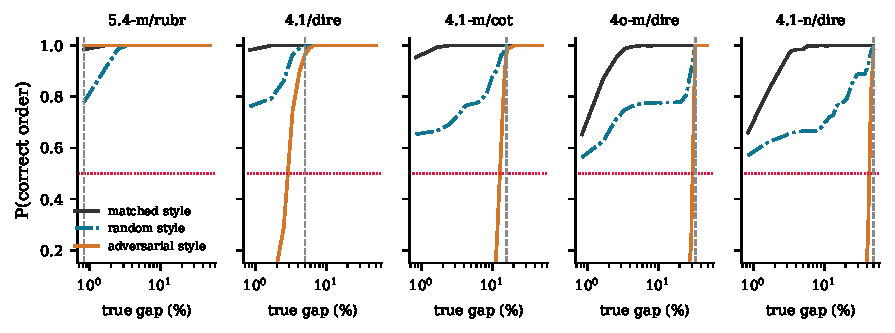
\includegraphics[width=\textwidth]{../figures/f2_curves.pdf}
\caption{Probability of correctly ordering two systems as a function of their true quality
gap (log axis), for five representative judges ordered by resolution limit. Black: both
systems rendered in the same style. Teal: styles assigned independently at random. Orange:
the worse system wears the judge's preferred style. Dashed grey marks the measured resolution
limit. \textbf{Takeaway:} the adversarial curve is a step, and its location---not the judge's
average accuracy---is what determines whether a leaderboard gap means anything.}
\label{fig:curves}
\end{figure}

\paragraph{Observation 3: limits vary by $60\times$; accuracy varies by $22$ points.}
We define a judge's measured resolution limit as the smallest gap beyond which adversarial
accuracy stays above $0.95$ for all larger gaps. Figure~\ref{fig:limits}(a) reports it for all
$28$ configurations. The best, \texttt{gpt-5.4-mini}/\textsc{rubric}, resolves $0.83\%$ of an
answer's factual content; the worst, \texttt{gpt-4.1-nano}/\textsc{direct}, needs $50\%$. The
median is $10.8\%$. Over the same pool, pooled meta-evaluation accuracy spans $66.1\%$ to
$88.3\%$.

\emph{Interpretation.} Accuracy and the limit are strongly related in rank order
($\rho=-0.89$), so accuracy is not uninformative---a hypothesis we entered with and
abandoned. But the accuracy scale is severely non-linear in the decision-relevant quantity: a
$22$-point accuracy range corresponds to a $60\times$ range in resolving power
(Figure~\ref{fig:limits}(b)). Reading "this judge scores $0.69$ and that one $0.88$" as a
modest difference is a serious misreading of what those numbers imply for a leaderboard.

\begin{figure}[t]
\centering
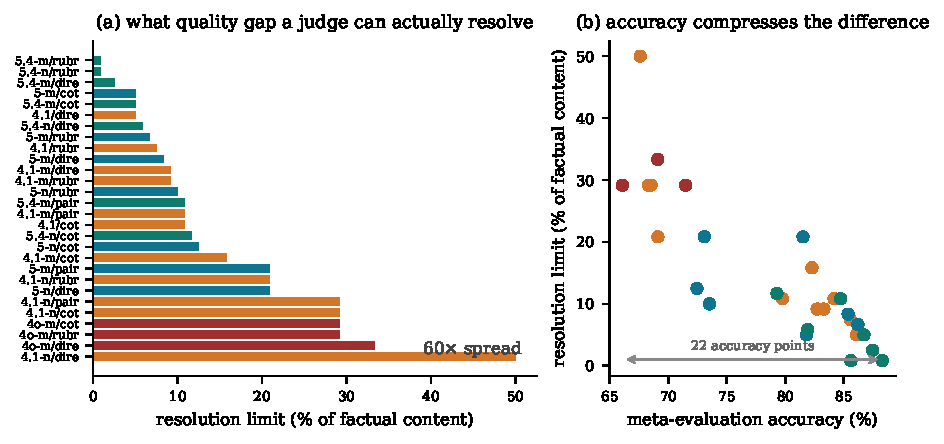
\includegraphics[width=\textwidth]{../figures/f1_limits.pdf}
\caption{\textbf{(a)} Measured resolution limit for all 28 judge configurations, coloured by
model family. \textbf{(b)} The same limits against pooled meta-evaluation accuracy.
\textbf{Takeaway:} the quantity that decides whether a leaderboard gap is meaningful varies by
$60\times$ across judges, and the accuracy scale compresses that into $22$ points.}
\label{fig:limits}
\end{figure}

\paragraph{Observation 4: verbosity preference is the norm, and it reverses at the frontier.}
Of $28$ configurations, $18$ score the \texttt{padded} style highest, $7$ \texttt{plain} and
$3$ \texttt{polished}, with the exceptions concentrated in the newest family. Protocol matters
as much as model: within \texttt{gpt-5.4-mini} the limit is $0.83\%$ under \textsc{rubric},
$2.5\%$ under \textsc{direct}, $5.0\%$ under \textsc{cot} and $10.8\%$ under pairwise.
\emph{Interpretation, offered cautiously:} our pairwise arm shows \emph{larger} style
sensitivity than pointwise scoring, which sits awkwardly beside
\citet{norman2026reliability}'s small ($<0.011$) verbosity bias under a pairwise rubric. Our
pairwise score is a win rate against a fixed anchor---a different estimator on a different
scale---so we flag this as needing direct study rather than treating it as a contradiction.

\section{What the meta-benchmark can and cannot tell you}
\label{sec:composition}

We expected the informativeness of pooled agreement to depend on how the meta-benchmark is
composed, and specifically that restricting it to clear-cut pairs---the standard design goal,
since ambiguous pairs are unreliable to annotate---would destroy the signal. \textbf{It does
not.} Recomputing accuracy under five compositions and correlating each with the resolution
limit gives $\rho$ between $-0.79$ and $-0.89$: full grid $-0.89$, clear-cut only
($|\Delta k|\ge3$) $-0.80$, style-matched pairs only $-0.87$, both restrictions $-0.79$,
near-ties only $-0.89$. The ordinal signal is robust.

The failure is not ordinal but \emph{metric} (Table~\ref{tab:calib}).

\begin{table}[t]
\caption{Predicting a judge's measured resolution limit $\rlim_J$. Residual standard deviation
is in units of true quality; lower is better. The gold-label predictors require an annotated
meta-benchmark; the bias-equivalent gap $\bgap_J$ requires no labels at all. $\rlim_J$ itself
is measured with labels---the point is that $\bgap_J$ recovers it without them.}
\label{tab:calib}
\centering
\begin{tabular}{llcc}
\toprule
Predictor & Labels needed & $R^2$ & Residual s.d. (\% of content) \\
\midrule
Accuracy, full composition            & gold & $0.723$ & $6.3$ \\
Accuracy, clear-cut pairs             & gold & $0.699$ & $6.6$ \\
Accuracy, style-matched pairs         & gold & $0.684$ & $6.7$ \\
Accuracy, clear-cut $+$ matched       & gold & $0.667$ & $6.9$ \\
Accuracy, near-ties only              & gold & $0.698$ & $6.6$ \\
\midrule
$\bgap_J$, bias-equivalent gap (ours) & \textbf{none} & $\mathbf{0.927}$ & $\mathbf{3.3}$ \\
\bottomrule
\end{tabular}
\end{table}

\emph{Interpretation.} A residual of $6.3\%$ of factual content exceeds the entire resolution
limit of the seven best judges in our pool. So a practitioner who knows a judge's meta-benchmark
accuracy still cannot answer the question they need answered---\emph{is my observed $5\%$
leaderboard gap real?} The label-free estimator halves that residual and is expressed directly
in the units of the question (Figure~\ref{fig:calibration}).

\begin{figure}[t]
\centering
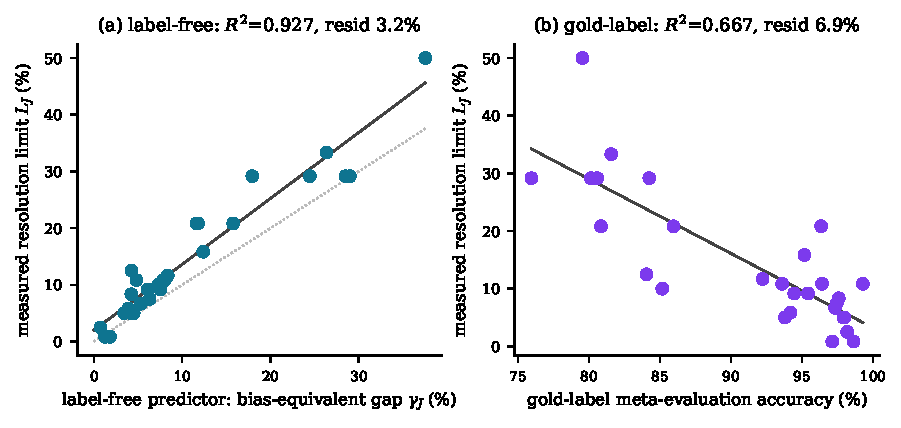
\includegraphics[width=\textwidth]{../figures/f3_calibration.pdf}
\caption{Recovering the resolution limit. \textbf{(a)} The label-free predictor $\bgap$;
dotted line is $y=x$. \textbf{(b)} Gold-label accuracy on a clear-cut, style-matched
meta-benchmark. \textbf{Takeaway:} both are informative, but only the label-free predictor is
calibrated well enough to convert into a decision about a specific leaderboard gap.}
\label{fig:calibration}
\end{figure}

\section{The certificate in the leaderboard regime}
\label{sec:certificate}

The regime that matters is the one leaderboards live in: systems separated by small margins,
each rendered in whatever style it happens to produce. We drew $4{,}000$ random system pairs
per judge with true quality gaps uniform in $(0.8\%,16.7\%]$ of factual content and styles
drawn independently, then applied Theorem~\ref{thm:cert}: certify the ordering iff
$|\Qhat(s)-\Qhat(s')|>R_J$, with $R_J$ measured with no labels.

\begin{table}[t]
\caption{Certificate performance, averaged over 28 judge configurations, $4{,}000$ pairs each.
The threshold $R_J$ is estimated from data, so the right-hand block re-estimates it on 42
items and evaluates on the disjoint 43. That split also halves the evaluation set, which
independently adds sampling noise to every system mean; the two effects are reported together
rather than disentangled.}
\label{tab:cert}
\centering
\begin{tabular}{lccc}
\toprule
& \multicolumn{2}{c}{all 85 items} & split-half \\
& Mean & Worst judge & Mean \\
\midrule
Ranking accuracy if you simply trust the judge & $0.860$ & $0.687$ & $0.838$ \\
Coverage (fraction of pairs certified)         & $0.558$ & --- & $0.571$ \\
Ranking accuracy on \emph{certified} pairs     & $\mathbf{0.969}$ & $0.834$ & $\mathbf{0.943}$ \\
Ranking accuracy on pairs it \emph{declines}   & $0.721$ & --- & $0.683$ \\
\bottomrule
\end{tabular}
\end{table}

\emph{Observation.} The certificate separates the trustworthy claims from the rest: accuracy
is $0.969$ on the pairs it certifies and $0.721$ on the pairs it refuses, a gap of $24.8$
points, at $55.8\%$ coverage and zero labelling cost. The separation is not an artefact of
estimating the threshold on the evaluation data: with $R_J$ estimated on a disjoint half of
the items, certified accuracy is $0.943$ against $0.683$ on the declined pairs, a gap of
$26.0$ points. For the strongest judge
(\texttt{gpt-5.4-mini}/\textsc{direct}) coverage reaches $97.2\%$ at $98.8\%$ accuracy; for the
weakest it correctly collapses to $12.5\%$ coverage, which is the right behaviour---a judge
that cannot resolve the gaps in question should certify almost nothing.

\begin{figure}[t]
\centering
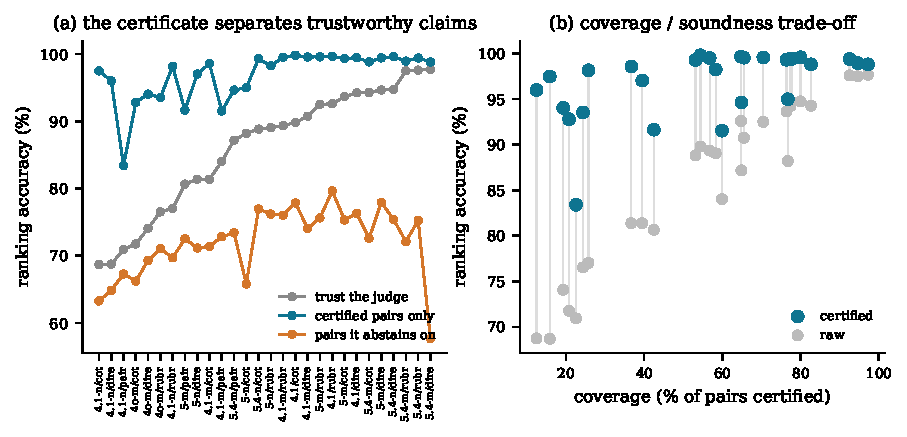
\includegraphics[width=\textwidth]{../figures/f4_certificate.pdf}
\caption{The certificate in the leaderboard regime (gaps $\le 16.7\%$ of factual content,
independent styles). \textbf{(a)} Judges sorted by raw accuracy. \textbf{(b)} Coverage against
accuracy. \textbf{Takeaway:} certified orderings are reliable across the whole judge pool, the
pairs the certificate declines are exactly the unreliable ones, and weak judges correctly
certify almost nothing.}
\label{fig:cert}
\end{figure}

\emph{Interpretation, including the shortfall.} Theorem~\ref{thm:cert} would give $100\%$
certified accuracy if $\delta$ were generated entirely by the style family. The observed
$96.9\%$ therefore \emph{measures} the residual differential bias $\delta_\perp$ orthogonal to
our three transformations. That $3.1\%$ is the price of a finite $\mathcal{T}$, and it is the
quantity a practitioner reduces by adding transformations. We prefer reporting it to
asserting a guarantee we have not earned.
\section{Real systems: the regime leaderboards occupy}
\label{sec:real}

Constructed systems buy exact ground truth; the objection is that they are not real ones. We
repeat the study with five models answering the same $85$ questions freely, quality
\emph{measured} as reference claims supported minus contradicted, restyled into the same three
styles so $R_J$ stays label-free (Appendix~\ref{app:real}).

Two caveats bound what this shows: measured quality is a coverage-weighted proxy (correlating
with length, $r=0.31$ item-level) and restyling moves it by $0.049$, so quality-preservation is
approximate rather than exact. \emph{Observation:} the five models span a measured quality
range of $\mathbf{0.108}$---almost exactly the median judge's resolution limit ($0.108$). Real
comparisons sit right at the edge of what these judges resolve, and it shows: judges agree with
measured quality at $\rho=0.85$ but with each other at only $\rho=0.70$, and raw ranking
accuracy on fine-grained pairs falls to $0.652$. The certificate still separates, $0.754$
certified against $0.584$ declined. \emph{Interpretation:} this is what the theory predicts for
a population separated by less than the resolution limit, and it is the ordinary case rather
than an adversarial one. With a noisy proxy and approximate quality-preservation the ceiling
here is well below one, so we read it as establishing \emph{which regime} real comparisons
occupy, not as a second validation of the certificate. Concretely: treat
Sections~\ref{sec:limits}--\ref{sec:certificate} as the evidence for the method, and this
section as evidence that the method is aimed at the right target.

\section{Where the regress terminates}
\label{sec:regress}

The worry motivating this paper is a regress: judges need meta-evaluation, meta-evaluation needs
meta-meta-evaluation, without ground. It terminates at L3, and Proposition~\ref{prop:decomp}
says why: \textbf{rankings depend only on quality differences, not levels}, and a transformation
with a known effect on quality supplies differences without naming a quality value. The claim is
about how grounding scales. L1 needs labels for every item; L2 needs a labelled meta-benchmark,
re-collected whenever the system population changes; L3 needs only that $\mathcal{T}$ is
quality-preserving---a fixed, reusable assumption about transformations we authored, $O(1)$ in
systems, judges and items. A level-4 question ("is $\mathcal{T}$ really quality-preserving?") is
one finite check, not a demand that grows with what is evaluated. The regress terminates because
the grounding requirement stops growing.

\section{Related work}

\paragraph{Meta-evaluation of judges.} LLM-as-judge and its biases were charted by
\citet{zheng2023judging}; benchmarks \citep{lambert2024rewardbench,tan2025judgebench,zeng2024llmbar},
surveys \citep{gu2024survey} and cross-task studies \citep{bavaresco2024llms} followed. The
closest empirical neighbour is \citet{norman2026reliability}: $21$ judges, $\sim$541k
judgements, universal $\kappa$ deflation, judge rankings shifting by up to $14$ positions across
meta-benchmarks. They establish that judge rankings are unstable; we ask what that costs at the
level of a system ranking, explain it via Theorem~\ref{thm:pooled}, and give a label-free
remedy. \citet{rao2026agreement} show five agreement statistics collapse to one value on binary
verdicts, but scope themselves to single-judge validation rather than system ranking;
Table~\ref{tab:calib} supplies that link. \citet{pooled2026leaderboards} independently argue
pooled reporting hides system-specific structure. Length bias in particular has a standing
correction \citep{dubois2024length}, and self-preference is documented
\citep{panickssery2024llm}.

\paragraph{Bounding judge bias.} \citet{feuer2026biasbounded} \emph{enforce} an average
bias-bound by modifying the evaluation; ours is a post-hoc certificate on an ordering already
produced, so the two compose. \citet{weng2026policy} are closest to our label-free diagnostic: a
Policy Invariance Score from certified-equivalent rubric rewrites. Their rewrites are certified
by three human annotators where ours are quality-preserving by construction, theirs are
rubric-side where ours are output-side, and---in their own words---they do not bound downstream
ranking error, which is the gap Theorem~\ref{thm:cert} fills. Perturbation and metamorphic
stress-testing \citep{judgeharness2026,perteval2024,singlechar2025} is our transformation
family's ancestry.

\paragraph{Benchmark validity.} A review of $445$ benchmark papers found only $16\%$ report
uncertainty estimates \citep{constructvalidity2025}; we bootstrap every headline number over
items. Validity audits \citep{toolcallingaudit2026}, older work on automatic-metric validity
\citep{reiter2018structured,chaganty2018price} and measurement modelling
\citep{jacobs2021measurement} frame the construct question that declaring $\mathcal{T}$
operationalises.

\section{Limitations}

\textbf{One provider.} All judges and all generation come from a single model family; no
Anthropic API key was available in our environment. Our claims concern the \emph{protocol}
rather than any vendor, and the pool spans a wide capability range, but we make no
cross-provider claim and replication there is the obvious next step.

\textbf{A narrow quality construct.} True quality here is the fraction of six atomic factual
claims that are correct. This is deliberate---it is the dimension along which ground truth is
\emph{constructible}---but our results speak to ranking on factual accuracy, not helpfulness,
style, or safety.

\textbf{Is restyling really quality-preserving?} A reader may hold that verbosity genuinely
degrades an answer, making \texttt{padded} not quality-preserving. We re-ran everything with
the length-matched family \{plain, polished\}: limits still span $35\times$ and the estimator
still recovers them ($R^2=0.876$, residual $2.5\%$; Appendix~\ref{app:restricted}). More
fundamentally, the framework \emph{requires} declaring $\mathcal{T}$, forcing an explicit
commitment to a quality construct rather than leaving it implicit. The certificate's $3.1\%$
shortfall from soundness measures confounds outside those transformations, reported not hidden.

\textbf{The real-system arm is weaker.} Section~\ref{sec:real} rests on a coverage-weighted
quality proxy and approximate quality-preservation; read it as showing which regime real
comparisons occupy, not as a second validation. A stronger test needs an independently
defensible quality construct---the problem that motivated construction-based ground truth.

\section{Conclusion}

Meta-evaluation asks how often a judge agrees with a label. Practitioners need to know whether
a leaderboard gap is real. We showed these come apart in a specific, measurable way: judges
have resolution limits varying $60\times$ across a single provider's model range, agreement
tracks those limits ordinally but compresses them into $22$ accuracy points and cannot be
converted into one, and a label-free perturbation estimator both predicts the limit
($R^2=0.93$) and certifies individual ranking claims ($0.860\to0.969$ accuracy at $55.8\%$
coverage). The practical recommendation is small and concrete: alongside judge accuracy,
report the judge's resolution limit in the units of your quality construct, and do not defend a
leaderboard gap smaller than it.

\bibliographystyle{plainnat}
\bibliography{references}


\appendix

\section{Proof of Theorem~\ref{thm:pooled}}
\label{app:proofs}

Fix a population containing systems $s_1$ (the better) and $s_2$, each evaluated on $n$
items. Suppose both have at least $m$ items carrying the same gold-label value $c$, and let
$H_1, H_2$ be those label-$c$ cell sets, $|H_1|,|H_2|\ge m$.

Let $\sigma$ be the transposition that exchanges the judge scores of one cell $x_1\in H_1$
and one cell $x_2\in H_2$, leaving all gold labels in place. Because $q(x_1)=q(x_2)=c$, the
multiset $\{(\qhat(x),q(x))\}$ over the whole evaluation set is unchanged by $\sigma$:
the pair $(\qhat(x_1),c)$ and the pair $(\qhat(x_2),c)$ simply trade positions. Hence
$M(\sigma J)=M(J)$ for every pooled metric $M$, and the group $G$ generated by all such
transpositions leaves $M$ invariant.

The system means are not invariant. Applying $\sigma$ changes
\[
\Qhat(s_1)-\Qhat(s_2) \;\longmapsto\; \Qhat(s_1)-\Qhat(s_2) - \tfrac{2}{n}\bigl(\qhat(x_1)-\qhat(x_2)\bigr).
\]
Choose $x_1$ to carry a high score and $x_2$ a low one, so each transposition strictly
decreases the gap by $\tfrac{2}{n}\Delta$ with $\Delta>0$ the within-label score spread
realised by that swap. Applying $t \le m$ disjoint such transpositions gives
\[
\Qhat(s_1)-\Qhat(s_2) \;=\; \bigl(Q(s_1)-Q(s_2)\bigr) + \bigl(\delta(s_1)-\delta(s_2)\bigr) - \tfrac{2t}{n}\bar\Delta ,
\]
where $\bar\Delta$ is the mean spread over the chosen swaps. Whenever
$\tfrac{2m}{n}\bar\Delta$ exceeds the initial gap, some $t\le m$ drives the difference
strictly negative, so the judge $J_2 = \sigma_t\cdots\sigma_1 J$ orders the pair wrongly while
$J_1=J$ orders it correctly. Both have identical $M$. Restricting the population to
$\{s_1,s_2\}$ gives $\SRA(J_1)=1$ and $\SRA(J_2)=0$. $\square$

Two remarks. First, the construction needs the judge to be non-constant within the label
class; a judge that assigns one value to every gold-$c$ item is unaffected, but such a judge
also carries no information beyond the label. Second, the theorem is about what a pooled
metric \emph{determines}, not about what is typical: it says the map from pooled metric to
ranking fidelity is not a function, so no refinement of the metric within the pooled frame
can make it one.

\section{Stimulus-integrity detail}
\label{app:integrity}

Full protocol of \citet{balli2026oracle}, run before any statistic was computed. Round~1 is
the initial build; round~2 is after the fix described in Section~\ref{sec:integrity}.

\begin{table}[h]
\caption{Stimulus-integrity checks. ``Verbatim copies'' counts answers that normalise to the
joined claim list, i.e.\ that were not rewritten at all.}
\centering\small
\begin{tabular}{lccccc}
\toprule
& \multicolumn{2}{c}{mean words} & \multicolumn{2}{c}{verbatim copies / 425} & claim \\
Condition & round 1 & round 2 & round 1 & round 2 & fidelity \\
\midrule
plain    & $77$  & $99$  & $325$ & $\mathbf{0}$ & $0.995$ \\
polished & $130$ & $130$ & $0$   & $0$          & $0.998$ \\
padded   & $286$ & $286$ & $0$   & $0$          & $0.995$ \\
\bottomrule
\end{tabular}
\end{table}

Mechanical no-op check: $0/510$ corrupted claims string-identical to their true counterpart,
under exact and whitespace-normalised comparison. This is the cheap oracle whose absence
\citet{balli2026oracle} identify as the structural weakness of LLM-generated-negative
corpora; because our corruption step is a claim substitution, it costs nothing here.
Fragments under three words: $0$ in all $15$ conditions. Rendering-level no-ops (an answer at
$k>0$ in which the checker detects no false claim): $5/1020$ ($0.5\%$), reported rather than
removed.

We also read $20$ raw items per condition by hand. One apparent fault turned out to be our own
misreading and is worth recording, since it illustrates why the manual pass is not optional in
either direction. In item \texttt{it0072} the corrupted claim ``The Flyer used a
12-horsepower gasoline engine built by the Wright brothers'' looked wrong, because $\sim$12
horsepower is historically correct. Inspecting the pair showed the horsepower is held constant
across both versions and the corruption is the \emph{builder} (Charlie Taylor $\to$ ``the
Wright brothers''): a correctly constructed minimal entity substitution. From an aggregate
view this is invisible; from the raw pair it takes ten seconds.

\section{Real-systems detail}
\label{app:real}

Five models (\texttt{gpt-4.1-nano}, \texttt{gpt-4o-mini}, \texttt{gpt-4.1-mini},
\texttt{gpt-5-nano}, \texttt{gpt-4.1}) answered the $85$ questions with no claim list and no
style instruction. A checker decided, for each of the item's six reference claims, whether the
answer supports, contradicts or omits it; measured quality is (supported $-$ contradicted)$/6$.
This is the only place in the project where ground truth is estimated rather than constructed,
and it is a narrow entailment check against a given claim rather than a holistic judgement.

Measured quality: \texttt{gpt-4.1-nano} $0.347$, \texttt{gpt-4o-mini} $0.378$,
\texttt{gpt-4.1-mini} $0.396$, \texttt{gpt-4.1} $0.408$, \texttt{gpt-5-nano} $0.455$. The
ordering is not the one model size would suggest, which is itself evidence that the proxy is
partly a coverage measure: it correlates with answer length at $r=0.54$ across models and
$r=0.31$ at item level. Restyling each answer into the three styles moved measured quality by
$0.049$ on average ($p95 = 0.167$); that figure mixes genuine content drift with checker noise,
and we cannot separate the two without repeated checks.

Eight judge configurations scored all $1{,}700$ records. Systems with arbitrarily fine quality
gaps come from mixing two models' answers item-by-item at rate $p$, giving quality
$(1-p)Q_A + pQ_B$.

\section{Error decomposition}
\label{app:decomp}

\begin{figure}[t]
\centering
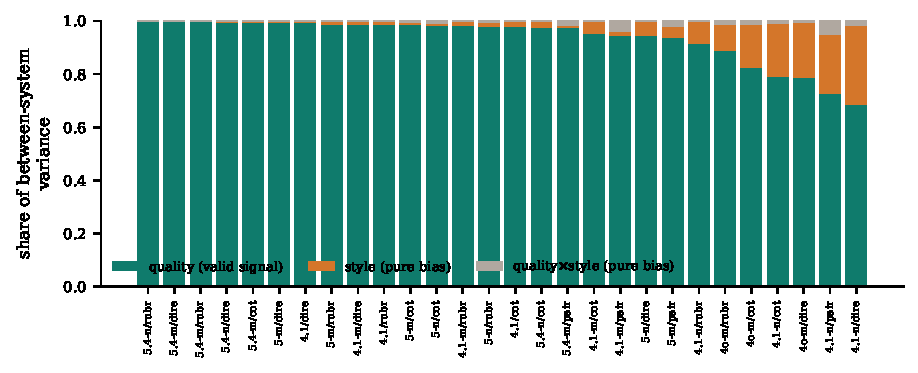
\includegraphics[width=\textwidth]{../figures/f5_decomposition.pdf}
\caption{Two-way ANOVA on each judge's system means. Because restyling preserves quality by
construction, the style and interaction components are pure bias and the quality component is
the only valid signal. \textbf{Takeaway:} at the coarse quality gaps of the original grid,
valid signal dominates for every judge---which is why ranking looks solved there, and why the
interesting question is what happens as the gap shrinks.}
\label{fig:decomp}
\end{figure}


\section{Judge prompts}
\label{app:prompts}

All three pointwise protocols present the question and the answer and ask for a line
\texttt{SCORE: <number>}. \textsc{direct}: ``Rate the overall quality of the following answer
\dots\ Give a score from 1 (very poor) to 10 (excellent).'' \textsc{rubric}: the same, prefaced
by ``Consider: factual accuracy---are the stated facts correct? completeness---does it cover
what the question asks? clarity---is it well written?'' \textsc{cot}: ``First reason briefly (at
most 80 words) about the answer's strengths and weaknesses. Then give an overall score\dots''
The pairwise protocol shows two answers to the same question and asks for
\texttt{VERDICT: A} or \texttt{VERDICT: B}; each pair is run in both orders against a fixed
anchor system ($k{=}2$, \textsc{plain}), and a system's score is its win rate against that
anchor. Unparseable outputs: $0$ of $30{,}600$ pointwise, $71$ of $9{,}520$ pairwise ($0.75\%$).

\section{Rendering fidelity, and whether it matters}
\label{app:fidelity}

The renderer is an LLM, so faithfulness is checked, not assumed. Across all $1275$ cells,
$7621/7650 = 99.6\%$ of claim slots assert the intended version. Aggregating to cells,
\textbf{28 of 1275 ($2.2\%$) contain at least one slot where the renderer silently repaired a
corrupted claim or dropped a true one}, so those cells' real quality differs from their intended
$Q=(6-k)/6$ by one claim out of six. The failures are spread over $15$ of the $85$ items and
across all three styles (\textsc{padded} 12, \textsc{plain} 11, \textsc{polished} 5).

Since every analysis uses the intended quality as ground truth, we checked whether this matters
by dropping all $15$ affected items and redoing the headline analysis on the remaining $70$.
The label-free predictor's recovery of the measured resolution limit is unchanged:
$\rho = 0.964$ and $R^2 = 0.942$ on the reduced set against $\rho = 0.932$ and $R^2 = 0.938$ on
the full set, with the predictor's ordering of judges essentially identical across the two
($\rho = 0.985$). The spread of resolution limits is $50\times$ rather than $60\times$, since
excluding items removes some of the extremes. We report the full-set numbers throughout and
regard the fidelity slippage as real but not load-bearing.

\section{Restricted transformation family}
\label{app:restricted}

A reader may hold that verbosity genuinely degrades an answer, so that our \texttt{padded}
transform is not quality-preserving and part of what we call bias is signal. We therefore
repeat the analysis with $\mathcal{T}'=\{\texttt{plain},\texttt{polished}\}$, which are close
in length ($99$ vs $130$ words) and differ essentially in formatting.

\begin{table}[h]
\caption{Restricted family $\mathcal{T}'$ versus the full family $\mathcal{T}$.}
\centering\small
\begin{tabular}{lcc}
\toprule
& $\mathcal{T}$ (3 styles) & $\mathcal{T}'$ (2 styles) \\
\midrule
Mean quality share of between-system variance & $0.935$ & $0.978$ \\
Minimum quality share over judges             & $0.684$ & $0.711$ \\
Spread of resolution limits across judges     & $60\times$ & $35\times$ \\
$\rho(\bgap,\ \text{limit})$ within family  & $0.936$ & $0.786$ \\
$R^2$ predicting the limit within family      & $0.927$ & $0.876$ \\
Residual s.d. (\% of factual content)         & $3.3$ & $2.5$ \\
\bottomrule
\end{tabular}
\end{table}

The phenomena survive: even with the disputed condition removed, resolution limits still span
$35\times$ and the label-free estimator still recovers them far more precisely than any
gold-label predictor does ($2.5\%$ residual against $\sim$$6.3\%$; Table~\ref{tab:calib}).

One cross-family result is worth stating because it could be mistaken for a failure. Using the
restricted estimator $\bgap^{\mathcal{T}'}$ to predict the \emph{full-family} limit gives
only $\rho=0.489$. This is the theory behaving as advertised rather than breaking:
Theorem~\ref{thm:cert} is sound relative to the declared family, and a family that contains no
verbosity contrast cannot bound a confound driven by verbosity. The estimator predicts exactly
the confounds it is asked about. The practical consequence is that $\mathcal{T}$ must be
declared, and declaring it is precisely the act of committing to a quality construct.

\end{document}
